%\documentclass[9pt, twoside, openright]{memoir}
\documentclass[9pt, a4paper, twoside, openright]{memoir}

\setstocksize{11in}{8in}
\settrimmedsize{9in}{7in}{*}
\settrims{0.7in}{.75in}
\settypeblocksize{7.5in}{6in}{*}
\setlrmargins{.85in}{*}{*}
\setulmargins{.5in}{*}{*}
\setheadfoot{\onelineskip}{2\onelineskip}
\setheaderspaces{*}{2\onelineskip}{*}

\checkandfixthelayout

\makeatletter
\DeclareOldFontCommand{\rm}{\normalfont\rmfamily}{\mathrm}
\DeclareOldFontCommand{\sf}{\normalfont\sffamily}{\mathsf}
\DeclareOldFontCommand{\tt}{\normalfont\ttfamily}{\mathtt}
\DeclareOldFontCommand{\tt}{\smallfont\ttfamily}{\texxttt}
\DeclareOldFontCommand{\bf}{\normalfont\bfseries}{\mathbf}
\DeclareOldFontCommand{\it}{\normalfont\itshape}{\mathit}
\DeclareOldFontCommand{\sl}{\normalfont\slshape}{\@nomath\sl}
\DeclareOldFontCommand{\sc}{\normalfont\scshape}{\@nomath\sc}
\makeatother

% \usepackage{xcolor, calc, graphicx, soul, fourier, verbments, makeidx, mflogo}
\usepackage{xcolor, calc, graphicx, soul, minted, makeidx, mflogo, 
  pstricks, minitoc, amsmath, amssymb, pst-poly, longtable, tikz}
\usetikzlibrary{shapes, arrows}
% Define block styles
\tikzstyle{decision} = [diamond, draw,
  text width=4.5em, text badly centered, node distance=3cm, inner sep=0pt]
\tikzstyle{startstop} = [rectangle, draw, 
  text width=5em, text centered, rounded corners, minimum height=2em]
\tikzstyle{line} = [draw, -latex']
\tikzstyle{cloud} = [draw, ellipse, node distance=3cm,
  minimum height=0.5cm]
\tikzstyle{io} = [trapezium, trapezium left angle=70, trapezium right
  angle=110, minimum width=0.5cm, minimum height=0.5cm, text centered, draw=black,
]
\tikzstyle{process} = [rectangle, minimum width=1cm, minimum height=0.5cm, text
  centered, draw=black]
\tikzstyle{arrow} = [->,>=stealth]

\let\footruleskip\undefined
\usepackage{fancyhdr}
\usepackage{fancyvrb}
\pagestyle{fancy}
%\usepackage[shellescape, latex]{gmp}
\showtrimson

\definecolor{niceblack}{rgb}{.1, .1, .1}
\definecolor{webred}{rgb}{.7,0,0}
\definecolor{webbg}{rgb}{1,.8,.2}
\definecolor{bootstrapurl}{rgb}{0,.5,.75}
%\definecolor{nicered}{rgb}{.347,.129,.149}
%\definecolor{nicegreen}{rgb}{.129,.447,.149}
%\definecolor{niceblue}{rgb}{0, 0, .6}
%\definecolor{niceyellow}{rgb}{1,1,.95}
%\color{niceblack}
\usepackage[colorlinks]{hyperref}
\hypersetup{%
  pdftitle={C Programming with C11},
  pdfauthor={Shiv S. Dayal},
  pdfkeywords={C, Programming},
  bookmarksnumbered,
  pdfstartview={FitH},
  urlcolor=niceblack,
  linkcolor=niceblack,
}%

\setlength{\tabcolsep}{10pt}
\renewcommand{\arraystretch}{1.5}

\renewcommand{\chaptermark}[1]{%
  \markboth{#1}{}}
\renewcommand{\sectionmark}[1]{%
  \markright{#1}{}}

\makeatletter
\newlength\dlf@normtxtw
\setlength\dlf@normtxtw{\textwidth}
\def\myhelvetfont{\def\sfdefault{mdput}}
\newsavebox{\feline@chapter}
\newcommand\feline@chapter@marker[1][4cm]{%
  \sbox\feline@chapter{%
    \resizebox{!}{#1}{\fboxsep=1pt%
      \colorbox{niceblack}{\color{white}\bfseries\sffamily\thechapter}%
  }}%
  \rotatebox{90}{%
    \resizebox{%
      \heightof{\usebox{\feline@chapter}}+\depthof{\usebox{\feline@chapter}}}%
              {!}{\scshape\so\@chapapp}}\quad%
  \raisebox{\depthof{\usebox{\feline@chapter}}}{\usebox{\feline@chapter}}%
}
\newcommand\feline@chm[1][4cm]{%
  \sbox\feline@chapter{\feline@chapter@marker[#1]}%
  \makebox[0pt][l]{% aka \rlap
    \makebox[1cm][r]{\usebox\feline@chapter}%
}}
\makechapterstyle{daleif1}{
  \renewcommand\chapnamefont{\normalfont\Large\scshape\raggedleft\so}
  \renewcommand\chaptitlefont{\normalfont\huge\bfseries\scshape\color{niceblack}}
  \renewcommand\chapternamenum{}
  \renewcommand\printchaptername{}
  \renewcommand\printchapternum{\null\hspace*{5.5in}\feline@chm[1cm]\par}
  \renewcommand\afterchapternum{\par\vskip\midchapskip}
  \renewcommand\printchaptertitle[1]{\chaptitlefont\raggedleft ##1\par}
}
\makeatother
\chapterstyle{daleif1}



\title{\HUGE{\textbf{Computer Programming with 
      GNU/Linux}}\\\vspace*{1cm}\Large{Vol. I}\\\vspace*{1cm}\HUGE{\textbf{C 
      Programming with C11}}\vspace*{2cm}}
\author{\vspace*{1cm}\LARGE{Shiv S. Dayal}}
\date{}

\renewcommand{\ttdefault}{pcr}
\setlength{\parskip}{1em}
%\renewcommand{\rmdefault}{ptm}
%\renewcommand{\rmdefault}{phv}
\renewcommand{\contentsname}{Table of Contents}
\makeindex
\begin{document}
\dominitoc
\dominilof
\dominilot
\maketitle
\thispagestyle{empty}
\pagestyle{empty}
\vfill
\newpage
\vspace*{7in}
Copyright, \copyright~ Shiv Shankar Dayal, 2011. All rights reserved.
\newpage
\vspace*{2in}
\begin{center}
  Dedicated to my family\\and Free Software Community
\end{center}
\newpage
\setcounter{page}{1}
\pagenumbering{roman}
\tableofcontents
\newpage
\listoffigures
\newpage
\listoftables
% \newpage
% \listofpyglistings
\newpage
\pagestyle{fancy}
\frontmatter
\setcounter{page}{1} 
\pagenumbering{roman}
\chapter{Preface}
I welcome you to this pdf version of 
\url{https://10hash.com/books/c/} which is a complete rewrite. That 
was my first attempt to write at such a large scale and therefore there were 
many deficiencies in that version which I hope have been countered and
corrected in this version. In the HTML version I had put a lot of emphasis on 
specification. However, the feedback which I got from some of my readers is 
that it has become complicated and is not suitable for beginners. After 
thinking over it I found that it is the order of chpaters which needs to be 
corrected and a lot more examples and exercises need to be there.

In this rewrite I will arrange the chapters in a different way. The empahsis on 
specification will be treated in the last part of book.

\section*{What this book contains?}
This book is about C programming language. In this book I have explained the
syntax of C programming language. But it is not only for learning about
language but how to learn to program using C programming language is also
there. In this book we will follow latest ISO specification of C which is
popularly known as C11.

\section*{Who should read this book?}
People interested in learning C should read this. Anybody can read this book
who has little background on Mathematics. I would say high school education is
sufficient for reading it. So this book is for both beginners and experts
alike. For experts advanced concepts have been presented and also a reference
to standard library has been given along with its usage.

\section*{How to read this book?}
Well, learning programming is like learning a new language and then solving
problems is like Mathematics. So the latter is more important as unless you can
solve the problem on pen and paper, you cannot solve the problems using
C. However, the focus of this book is to explain the features and syntax of C
programming language not on how to solve the problem. To get a good grasp
on the contents of the book one should read the theory first then look at the
examples given and try to understand and run them and in the end attempt
the problems. If you cannot solve the problems then lookup the solution and
try to understand. In case of any problem please log on to my personal
question/answer website \url{http://kunjika.libreprogramming.org/} to get
more help.

\section*{Acknowledgements}
I am in great debt of my family and free software community because both of
these groups have been integral part of my life. Family has prvided direct
support while free software community has provided the freedom and freed me
from the slavery which comes as a package with commercial software. I am
especially grateful to my wife, son and parents because it is their time which
I have borrowed to put in the book. To pay my thanks from free software
community  I will take one name and that is Richard Stallman who started all
this  and is still fighting this never-ending war. When I was doing the Algebra
book then I realized how difficult it is to put Math on web in HTML format and
why Donald Knuth wrote \TeX{}. Also, \TeX{} was one of the first softwares to
be released as a free software. HTML has not yet matured to represent
mathematical content. MathML is supported by Mozilla. Webskit browsers started
supporting  then dropped and I would refrain to comment on commercial browser's support which do not even comply to starndard because they think they are the standards tehmselves and others will bend to their will.

Now as this book is being written using \LaTeX{}~ so obviously Leslie Lamport
and all the people involved with it have my thanks along with Donald Knuth. I
use Emacs with Auctex and hope that someday I will use it in a much more
productive way someday.

I have used TikZ as a tool for drawing all the diagrams. It is a wonderful
package and works very nicely. I have great appreciation for its author Till
Tantau.

%For syntax highlighting I have used \texttt{Verbatim} \LaTeX{} package which
%uses \texttt{pygments} as its backend. You can modify it and make it look
%different both at \LaTeX{} and \texttt{pygments} level. Thanks to the
%respective package authors.

For errors and suggestion please email me at
\href{mailto:shivshankar.dayal@gmail.com}{shivshankar.dayal@gmail.com} where I
will try to respond to each mail as
much as possible. Please use your real names in email not something like
coolguy. As an alternative you can report it at
\url{https://10hash.com} where a question/answer website is maintained.
\begin{flushright}
Shiv Shankar Dayal\\
Nalanda,\\
India, 2015
\end{flushright}

\newpage
\mainmatter
\pagenumbering{arabic}
\chapter{Basics of C}
There are certain rules in every language, certain grammar which dictates the
way language will be spoken and written. It has a script to write
using. Similarly, programming languages have BNF (Backus-Naur Form)
context-free grammar. There are valid characters in a programming language and
a set of keywords. There are constructs to handle control flow, loops
etc. There are facilities provided by language to deal with numbers and strings
separately, to reuse the code and some basic data structures to facilitate
programming. However, programming language ruleset is very small compared
to a natural programming language. Also, when using natural programming
language like talking to someone or writing something the other person can
understand your intent but in programming you cannot violate rules. The grammar
is context-free. Compilers or interpreters cannot deduce your intent by reading
code. They are not intelligent. You make a mistake and it will refuse to listen
to you no matter what you do. Therefore, it is very essential to understand
these rules very clearly and correctly.

\section{The C Character Set}
The following form the C character set you are allowed to use in it:

\begin{verbatim}
[a-z] [A-Z] [0-9] ~ ! # % ^ & * ( ) - = [ ] \ ; ' , . / _ + { } | : " < > ?
\end{verbatim}
\index{character set}

This means along with other symbols you can use all English alphabets (both
uppercase and lowercase) and Arabic numerals. Symbols like \texttt{\$} and
\texttt{@} are not part of C's character set. But strings can contain any
these characters also. Strings are sequence of characters with double quotes
and double quotes iteself are escaped with \texttt{$\backslash$}. Also,
\texttt{\$} and \texttt{@} can also be value of characters. Characters are
values containing single characters withing single quotes. We will see more of
these in their individual sections. However, English is not the only
spoken language in the world. Therefore in other non-English speaking counties
there are keyboard where certain characters present in above set are not
present. The inventors of C were wise enough to envision this and provide the
facility in form of trigraph sequences. Given below is the trigraph sequence
table:

\begin{table}
 \begin{center}
 \caption{Trigraph Sequences}
\begin{tabular}{|c|c|c|c|c|c|}
\hline
\textbf{Trigraph}&\textbf{Equivalent}&\textbf{Trigraph}&\textbf{Equivalent}&\textbf{Trigraph}&\textbf{Equivalent}\\
\hline
??=&\#&??'&\textasciicircum&??!&|\\
\hline
??(&[&??)&]&??$<$&\{\\
\hline
??$>$&\}&??/&\textbackslash&??-&\textasciitilde\\
\hline
\end{tabular}
\end{center}
\end{table}
\index{trigraph sequences}

However, you should refrain from using trigraph sequences for portability 
reasons as suggested by GNU coding standards.

\section{Keywords}
The following are reserved keywords for C programming language which you are not 
allows to use other than what they are meant for:
\index{keywords}
\begin{table}[H]
 \begin{center}
  \caption{Keywords of C}
  \begin{tabular}{l l l l l}
    auto & break & case & char & const\\
    continue & default & do & double & else\\
    enum & extern & float & for & goto\\
    if & inline & int & long & register\\
    restricted & return & short & signed & sizeof\\
    static & struct & switch & typedef  & union\\
    unsigned & void & volatile & while & \_Bool\\
    \_Complex & \_Imaginary & &\\
  \end{tabular}
 \end{center}
\end{table}

These keywords are special in C as said and cannot be used for variable names 
or funciton names or otherwise other than in strings and comments.

\section{Identifiers}
The names which we give to our variables are known as identifiers. Something 
with which we identify the variables. As you have already seen what is allowed 
in C's character set but not all are allowed in an identifiers name. Only 
alphabets from English language both lowercase and uppercase, Arabic digits from 
zero to nine and underscore (\_) are allowed in an identifiers name. The rule 
for constructing names is that among the allowed characters it can only begin 
with only English alphabets and underscore. Numbers must not be first character. 
For example, \texttt{x, \_myVar, varX} and \texttt{yourId78} are all valid 
names. However, take care with names starting from underscore as they are mostly 
used by different library authors. Invalid identifier examples are \texttt{9x, 
my\$} and \texttt{your age}. Please read this section carefully and make sure 
understand the rules for naming identifiers. Later at the end of chapter there 
are some simple problems to practice with.

\section{Programming}
Let us revisit our first program and try to understand what it does. Here I am 
giving code once again for quick reference:

\begin{minted}{c}
// My first program
/* Description: This program does nothing.*/

#include <stdio.h>

int main(int argc, char* argv[])
{
  return 0;
}
\end{minted}

You can now issue a command as \texttt{\$gcc nothing.c} where 
\texttt{nothing.c} is the filename by which you saved the source code. Note 
that \texttt{\$} is the prompt not part of command itself. Then you can do an 
ls and you will find that \texttt{a.out} is a file which has been produced by 
clang. Now you can run this program by saying \texttt{\$./a.out} and nothing 
will happen. But if you type \texttt{\$echo \$?} then you will find that 0 is 
printed on screen which is nothing but 0 after \texttt{return} of our program.

As you can see this program does almost nothing but it is fairly complete 
program and we can learn a lot from it about C. Let us try to dissect it line
by line. The first line is a comment. 
Whenever C compiler parses C programs and it encounters \texttt{//} it ignores 
rest of line as code i.e. it does not compile them. This type of single line 
comment were introduced in C99 standard and if your compiler is really old the 
compiler may give you error message about it. The second line is
also comments. Anything between \texttt{/*} and \texttt{*/} is ignored like 
\texttt{//}. However, be careful of something like \texttt{/* some comment */
  more comment */}. Such comments will produce error messages and your program
will fail to compile. The reason for this is when first \texttt{*/} is
encountered by parser or compiler it will complete its token for the comment
and then further portion which we intented to be part of comment will cause
syntax error. 

Comments are very integral part of programming. They are used to describe 
various things. You can write whatever you want. They may also be used to 
generate documentation with tools like doxygen. Typically comments should tell
what the program is doing not how. Sometimes how can be covered, when the logic
is really complex. One should be generous while commenting the code.

The next line is \texttt{\#include <stdio.h>}. \texttt{\#include} is a
preprocessor directive. The preprocessor directive is handled by the C
preprocesor which is handled by C preprocessor which looks in four directories
for include files. The include filename comes after \texttt{\#include} either in
angular brackets or double quotes. The C preprocessor looks for these at four
different places at least out of which one or posiibly two is of interest for
now as we are dealing with angular brackets. Depending on the way your compiler
is installed the file \texttt{stdio.h} may be in \texttt{/usr/include} or
\texttt{/usr/local/include} but then again it may be in a non-standard path
also although possibility of that is very less and then it is controlled by
parameters whose discussion is beyond the scope of book. Let us say
\texttt{stdio.h} is present in either of aforementioned directories then the C
preprocessor will copies the contents and pastes them in source file along the
way putting \texttt{\#line} macros which are used for debugging
purposes. \texttt{\#line} macro is discussed later in the chapter which deals
with macros. You can see the output of C preprocessor by typing \texttt{\$gcc
  -E nothing.c} since it will scroll a lot on you terminal you can use a pager
like \texttt{less} to read it. The \texttt{-E} tells \texttt{gcc} to just allow
preprocessoing and not compile and link the file.

I have recorded a video on basics of compilation which you can see at
\url{http://www.youtube.com/watch?v=ARsoVgknRU0}.

Next line is \texttt{int main(int argc, char* argv[])}. Now this is very special
function. Every complete executable(shared objects or dlls or archive
libraririe do not have main even though they are C programs) C program will
have one main function unless you do assembly hacking. This function is where
the programs start. The first word \texttt{int} is a keyword which shirthand
for integer. This signifies the return type of function. \texttt{main} is the
name of the function. Inside parenthesis you see \texttt{int argc} which tells
how many arguments were passed to program and is short form of argument
count. While \texttt{char* argv[]} is a pointer to array which we will see
later. For now let us just remember that it holds all the arguments to the
program including the program name.

Next is a brace. The scope in C is determined by braces. Something outside any
brace has global scope (we will see these later), something inside first level
of brace has function or local scope. Something inside second or more level of
braces have got that particular block scope. Scope here means that when there
will be a closing brace that particular variable which is valid in that scope
will cease to exist. However, we do not have to worry about that yet as we do
not have any variable. Just note that a corresponding closing brace will be the
end of main function. For every opening brace which starts a scope a closing
brace is mandatory.

Next line is \texttt{return 0;} This means whoever has called \texttt{main()}
will get a 0 as \texttt{return} is returning 0. In this case, receiver is the
shell or operating system 
which has invoked the very program. The semicolon is called the terminator and
used also on Java or C++ for example. The very requirement of semicolon is to
terminate the statement and move on to next statement.

However, the program shown does not do much. Let us write a program which has
some more functionality and we can explore more of C. So here is a program
which takes two integers as input from users and presents their sum as
output. Here is the program:

\begin{minted}{c}
// My second program
// Author: Shiv S. Dayal
// Description: It adds two numbers

#include <stdio.h>

int main()
{
  int x=0, y=0, sum=0;

  printf("Please enter an integer:\n");
  scanf("%d", &x);

  printf("Please enter another integer:\n");
  scanf("%d", &y);

  sum = x + y;

  printf("%d + %d = %d\n", x, y, sum);

  return 0;
}
\end{minted}
and the output is:
\begin{verbatim}
shiv@shiv:~/book/code$ ./addition
Please enter an integer:
7
Please enter another integer:
8
7 + 8 = 15
shiv@shiv:~/book/code$
\end{verbatim}

Note that \texttt{shiv@shiv:~/book/code\$} is the prompt.

Let us discuss new lines one by one. The line \texttt{int x=0, y=0, z=0;} is
declaration and definition or initialization of three ints. \texttt{int}
keyword in C is used to represent integers. Now we have three integers with
there values set to 0. Note that how the variables are separated by commas and
terminated by semicolon(as we saw in last program also). We could have also
written it like this:

\begin{minted}{c}
int x;
int y;
int z;

x = 0;
y = 0;
z = 0;
\end{minted}

or

\begin{minted}{c}
int x, y, z;

x = y = z = 0;
\end{minted}

However, the first method is best and most preferred as it prevents use before
definition. \texttt{int} is a data-type in C. \texttt{x, y,} and \texttt{z} are
called variables of type \texttt{int}. This means that the size of these
variables will be same as \texttt{int}. Note that 
C is a statically typed language and all types have predefined memory
requirements. In cour case, \texttt{int} requires 4 bytes on 32-bit and 64-bit
systems but 2 bytes on 16-bit systems.

Here I have created a video about variables of C which you can see at
\url{http://www.youtube.com/watch?feature=player\_embedded\&v=6whuGZwv2-k} and
you can watch another about \texttt{printf} and \texttt{scanf} at
\url{http://www.youtube.com/watch?feature=player\_embedded\&v=U3jCSTR7Ulo}.

Let us learn a bit about \texttt{printf}. This function is declared in
stdio.h. The prototype of \texttt{printf()} is

\begin{minted}{c}
int printf(const char *restrict format, ...);
\end{minted}

The first argument format is what we have in first two function calls. The
second is a \texttt{...} which means it can take variable number of arguments
known as variable-list. We have seen this in the third call.This means it will
take a string with optional variable no. of arguments. The string is called the
format-string and determines what can be printed with supplied arguments. These
\texttt{...} are used to supply variable no. of arguments. In the first two
\texttt{printf()} statements we just print the format-string so that is
simple. However, in the last one, we have format as \texttt{\%d} which
signifies a decimal integer. The integers printed are in the same order in
which they were supplied.

\texttt{scanf()} is scan function which scans for keyboard input. As by now you
know that \texttt{\%d} is for decimal integer but we have not said \texttt{x}
or \texttt{y}. The reason is \texttt{x} and \texttt{y} are values while
\texttt{\&x} and \texttt{\&y} are the addresses of \texttt{x} and \texttt{y} in
memory. \texttt{scanf()} needs the memory address to which it can write the
contents to. You will see \texttt{\&} operator in action later when we deal
with pointers. Just remember for now that to use a simple variable with
\texttt{scanf()} requires \texttt{\&} before its name.

Till now we have just seen only \texttt{int} data-type but then there are more
data types for other types of numbers, characters and strings. Let us see them
one by one.

\section{Data Types}
What are data types? Why C needs data types? C is a statically typed language
that is every variable has a type associated with it. These types determine
what kind of values these variables can hold and how they will be interpreted.
When everything is a voltage level why not just deal with 0s and 1s? The answer
is simple. You need to abstract and segregate how much is required. For
example, say you are given a sequence of 0s and 1s how much can you work with
them. We as humans are not very versed with 0s and 1s. Also, say we encode
character `A' for 10101 will it be easy for you to see A or numbers. Also,
numbers range from $-\infty$ to $\infty$. Also, since C is statically typed the
sizes of data types have to be known at compile time. There are four types of
data types. Integral, floating-point, arrays and pointers. Here, I will deal
with the two former types and leave latter two for later. The integral types
are \texttt{char, short int, int, long} and \texttt{long long} and
floating-point types are \texttt{float, double} and \texttt{long
  double}. \texttt{signed} and \texttt{unsigned} are sign modifiers which also
modified the range of data types but do not affect their memory
requirements. By default all basic data types are \texttt{signed} in nature and
you must qualify you variables with \texttt{unsigned} if you want that
behavior. \texttt{short} and \texttt{long} are modifiers for size which the
data type occupies but I consider them as different types because memory
requirements are different. The ranges of integral data types directly reflect
their memory requirements and if you know how much memory they are going to
occupy you can easily compute their ranges. The range of floating-point comes
from IEEE specification. IEEE standard document 754 governs the binary
representation of floating point numbers which you can read at
\url{http://www.eecs.berkeley.edu/~wkahan/ieee754status/IEEE754.PDF}. This is
not available from IEEE website itself as they sell the specification's
electronic copies.

Let us write a program to find out ranges for integral data types:

\begin{minted}{c}
// Description: It gives ranges of integral data types

#include <stdio.h>
#include <limits.h>

int main()
{
  printf("Size of char is..........%d\n", sizeof(char));
  printf("Size of short int is.....%d\n", sizeof(short int));
  printf("Size of int is...........%d\n", sizeof(int));
  printf("Size of long is..........%d\n", sizeof(long));
  printf("Size of long long is.....%d\n", sizeof(long long));
  printf("Size of float is.........%d\n", sizeof(float));
  printf("Size of double is........%d\n", sizeof(double));
  printf("Size of long double is...%d\n", sizeof(long double));c

  return 0;
}
\end{minted}

Here \texttt{sizeof} is a compile time operator which computes size of any type
passed to it as an argument. So it is computing sizes of all the data types as
shown in the program. The output is given below:

\begin{verbatim}
Size of char is..........1
Size of short int is.....2
Size of int is...........4
Size of long is..........8
Size of long long is.....8
Size of float is.........4
Size of double is........8
Size of long double is...16
\end{verbatim}

Please note that the output shown is on 64-bit machine and it will be different
on 32-bit machines.
\chapter{Console I/O}
IO stands for input/output. C provides only mechanism to interact through
console using its standard library. C does not provide ways to have GUI
although that is possible with various GUI libraries most notable being
GTK. However, discussing about GTK is out of scope of this book. In this
chapter we will focus on console output facilities of C because any program we
write at this stage will be meaningless if it has no input/output. Typically
when we interact with a C program we give input using keyboard which is also
referred as \texttt{stdin} stream. The output is monitor or \texttt{stdout}
stream. There is one more stream \texttt{stderr} which is generally redirected
to monitor or a log file. For historical reasons these are known as
\texttt{FILE} stream which represents the datatype of these
streams. \texttt{FILE} is capable of representing other streams which are disk
based for example a file on your hard drive. There are more type of input
devices on a modern computer. For example, network i/o is there. Whenever you
browse web or download a file through your intenet connection network i/o comes
into play. There is an opengroup
which specifies functions for network related functions. Operating systems
like GNU/Linux are POSIX compatible which defines how network i/o will be
used. Even a printer is a special output device, a camera input, speakers
output, microphone input and so on. In this books we are concerned with
keyboard input, output on monitor and i/o using files. Other types of i/os are
out of scope of this book.

However, before we go on with i/o I would
like to present C's memory model which will be needed by our discussion of i/o
related functions. However, if things do not make sense even then please go
through it and come later to understand more. 

\section{C's Memory Model}
As you may be knowing RAM(random acess memory) is the area which is used as
primary memory. Whenever we execute a program the first thing which happens is
that it gets loaded into memory. Now a binary program becomes a process when it
is running i.e. a running program is referred as process. All processes have
memory area divided into different portions. These portions are known as data
segment, stack and code or text segment. Dats segement is further split in
three parts; initialized data segment, uninitialized data segment or BSS which
is name after an ancient assembler Block Started by Symbol and
heap. Initialized data segment contains initialized global variables and static
variables. For uninitialized data segment it is same as above just that the
variables are not initialized explicitly but implicitly to zero.

Heap is the largest area of memory used for dynamic memory allocation. As
you will see later that you can manage heap using \texttt{malloc(), calloc(),
realloc(),} and \texttt{free()}. Note that operating system does not manage memory
allocated for you on heap. You, the programmer, are responsible for allocating and
freeing up memory in area. If heap gets full os will use virtual memory or swap
space on hard disk. Objects allocated on heap persist across function
calls. However, there are some very nasty problems, which, come in picture when
you use heap. There are several of them. You may forget to allocate memory and
may dereference unallocated pointer. You may have initialized it to
\texttt{NULL} and try to dereference that. You may allocate and free twice. You
forgot to set pointer to \texttt{NULL} after freeing it. And last but not the
least you loose all pointers to the memory area before you can free. The nature
with this particular problem is that if your program is going to run for long
time then it is going to consume more and more memory. Because of its nature it
is known as memory leak. It is very difficult to detect such problems in code
which does not run for long periods of time. Our friend valgrind will come to
help up with this problem. When a memory leak happens it eats up RAM slowly and
then operating system has to use virtual memory as explained above. In a
nutshell, I will say that heap means you have to manage it.

\begin{figure}[t!]
\begin{center}
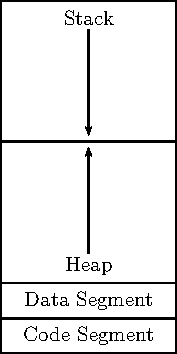
\includegraphics{figs/mem_model.pdf}
\end{center}
\caption{Memory model of a C program}
\end{figure}

Stack is relatively simple. All non-static and non-register variables go on
stack if not allocated dynamically. Stack variables do not retain there value
across function calls unless
they are passed as pointers. Also, when they go out of
scope, that is the scope in which they were declared ends, they will be kind of
lost. The way in which stack frame moves the same area will be used for new
variables. However, stack is very limited (compared to heap) and in deeply
nested function calls or recursion (you will see these in Functions chapter)
stack may get full and program may crash. The reason for crashing is that
operating system will not use virtual memory but will do a segmentation fault
in its place. GNU/Linux allow its users to modify the stack size by ulimit
command. Note that stack and heap are adjacent in memory and grow in opposite
direction.

Code segment or text segment is an area where the executable instructions of
program reside. It is typically constant and read-only area unless your system
allows self-modifying code. Following diagram shows the memory layout.

Note that this memory model not only applies to C but any process.

Now we will look at those functions, which, allow us to do console i/o. We will
begin with our familiar friends; printf and scanf.

\section{printf}
The prototype of \texttt{printf} is given by

\begin{Verbatim}[frame=single]
int printf(const char* fmt, ...);
\end{Verbatim}

Let us take a minute to understand this as we have not yet covered
functions. The first word is \texttt{int} which denotes the return type of the
\texttt{printf} function. This is no. of characters printed. Then we have name
of the function. \texttt{fmt} is the format string of type \texttt{const
 char}. In C, strings are either character arrays or character pointers. Here,
const means \texttt{printf} will not modify the format string. The ... means
variable no. of arguments, which, can be 0 also to be supplied to
\texttt{printf}.

\texttt{printf} is a string based output function that is It writes character
strings to \texttt{stdout}. The data which has to be written is formatted by
format string as shown previously. After the format specifier it expects as
many arguments as specified in format string. The characters which are not
like, say \texttt{\%d} for example, arecalled ordinary characters. These are
simply copied to output stream, which, is stdout for printf. The \texttt{\%d}
like conversion charcaters are known as conversion specification or format
specifiers. Each conversion specification should be augmented with one one
argument. The results are undefined if there are insufficient arguments for the
format. If extra arguments are given the excess arguments will be evaluated but
are otherwise ignored. However, there is a big problem here! There is no
type-safety. In general compiler will warn you about it and you, the
programmer, are responsible for giving correct format string, correct no. of
correct type of arguments. Consider the following program for example:

\begin{Verbatim}[frame=single]
#include <stdio.h>

int main()
{
  printf("%d %d\n", 3, 8);

  //do not mess it. undefined behavior
  printf("%d %d\n", 5);

  //extra arguments ignored
  printf("%d %d\n", 3, 5, "hello");

  //legal because char is integer type
  printf("%d\n", 's');

  //wrap around of integer as char
  printf("%c\n", 836);

  //do not mess with type-safety
  int i = printf("%d\n", "hello");
  prinf("%d\n", i);

  return 0;
}
\end{Verbatim}

now that if you give the command like \texttt{gcc -Wall printf.c} where
\texttt{printf.c} is the name of the ile then you will be shown following
warnings:

\begin{Verbatim}[frame=single]
printf.c: In function 'main':
printf.c:8:3: warning: format '%d' expects a matching 'int' argument [-Wformat=]
   printf("%d %d\n", 5);
   ^
printf.c:8:3: warning: format '%d' expects a matching 'int' argument [-Wformat=]
printf.c:11:3: warning: too many arguments for format [-Wformat-extra-args]
   printf("%d %d\n", 3, 5, "hello");
   ^
printf.c:11:3: warning: too many arguments for format [-Wformat-extra-args]
printf.c:20:3: warning: format '%d' expects argument of type 'int', but
argument 2 has type 'char *' [-Wformat=]
   int i = printf("%d\n", "hello");
   ^
printf.c:20:3: warning: format '%d' expects argument of type 'int', but
argument 2 has type 'char *' [-Wformat=]
\end{Verbatim}

Clearly this is not a good sign for any program. A program should compile
cleanly. In our case \texttt{gcc} is generating binary even though there are
warnings. You can make \texttt{gcc} generate more warnings by issuing a
\texttt{-Wall} flag. You can also treat all warnings as errors by passing
\texttt{-Werror} to \texttt{gcc}. These two options will ensure that your code
has no warnings. Now let us move to output and try to understand it. The output
on my system is as given below. It may differ on your system:
\\\\\texttt{3 8\\
5 8\\
3 5\\
115\\
D\\
134514119\\
10\\\\}
First \texttt{printf} is correct as expected. The second line causes undefined
behavior. You may think it is the previous 8 but believe me it is not
guaranteed that it will always the case. Ii is \textbf{UNDEFINED}. Third
\texttt{printf} is also fine in the sense that extra argument is
ignored. Fourth and fifth are normal. Sixth is again a big problem. You are
trying to print a decimal integer while argument is a character string. There
is no way for compiler to determine that what should be printed which will fit
on standards.

A full detail of all conversion specification is given in specification at \S(iso.7.21.6).

In real-world most of the time the conversion specifiers are kept simple. Given
below is a sample program showing some of the things given above:

\begin{Verbatim}[frame=single]
#include<stdio.h>

int main()
{
  int i   = 343456;
  float f = 123;
  long double ld = 78939.9347;

  printf("% d\n", i);
  printf("%+d\n", i);
  printf("%#o\n", i);
  printf("%#f\n", f);
  printf("%-08i\n", i);
  printf("%08i\n", i);
  printf("%8i\n", i);
  printf("%hhi\n", i);
  printf("%hi\n", i);
  printf("%li\n", i);
  printf("%lli\n", i);
  printf("%ji\n", i);
  printf("%zi\n", i);
  printf("%ti\n", i);
  printf("%8.8f\n", f);
  printf("%8.8Lf\n", ld);

  return 0;
}
\end{Verbatim}

The output of the above program is:
\\\\\texttt{ 343456\\
+343456\\
01236640\\
123.000000\\
343456\\
00343456\\
  343456\\
-96\\
15776\\
343456\\
4638355772471066016\\
4638355772471066016\\
343456\\
343456\\
123.00000000\\
78939.93470000\\\\}
We will keep seeing more conversion specifiers being used as we progress
through this book.

\section{scanf}
It scans \texttt{stdin} or keyboard for input. Its signature is same as that of
\texttt{printf()}. It reads bytes from keyboard input, interprets them
according to format string. It also expects a set of pointer arguments as
opposed to values for printf(). The pointers indicate where the interpreted
data from the input will be stored. The result is \texttt{UNDEFINED} if there
are less number of pointer arguments than the number of conversion specifers in
format string. Excess arguments will be evaluated but ignored. The format
string can have only white-space characters or an ordinary character (neither
`\%' nor a white-space character) or a conversion specification. Each
conversion specification is introduced by `\%', after which the following
appear in sequence.

For now if you do not understand what is a pointer then let us have a simple
definition for that. A pointer is a variable which stores a memory location
where the value will be stored.

Now that we have seen this description let us take a look at few examples.

\begin{Verbatim}[frame=single]
#include <stdio.h>

int main()
{
  char str[128] = {0};

  scanf("%s", str);
  printf("You entered:\n%s\n", str);

  return 0;
}
\end{Verbatim}

and the output is:
\\\\\texttt{\textbf{Hi! My name is Shiv.\\}
You entered:\\
Hi!\\\\}
It is certainly not the correct output. We had expected to see like: ``Hi! My
name is Shiv.''. What happend to input string after ``Hi!''. Well, in a form
given above for \texttt{scanf()} it will stop taking input after white-space
for character strings. For numerics it does not matter as it does not match the
format. For characters it is character-by-character so no confusion either. So
what if you want to have the entire string including white-spaces. Use
\texttt{[\^{}n]} as given below:

\begin{Verbatim}[frame=single]
#include <stdio.h>

int main()
{
  char str[128] = {0};

  scanf("%[^\n]s", str);
  printf("You entered:\n%s\n", str);

  return 0;
}
\end{Verbatim}

and the output is:
\\\\\texttt{\textbf{Hi! My name is Shiv.}\\
You entered:\\
Hi! My name is Shiv.\\\\}
What if you want to filter a string based on certain patterns. For example, a
charcater string does not contain more that a single space, English alphabets,
period and digits. To scan such a string you can define a pttern as program
given below shows:

\begin{Verbatim}[frame=single]
#include <stdio.h>

int main()
{
  char c[100]={0};

  scanf("%[ A-Za-z0-9!.]", c);
  printf("%s\n", c);

  return 0;
}
\end{Verbatim}

and the output is:
\\\\\texttt{\textbf{Hi! My name is Shiv! My phone no. is 1234. \%\^\$\&\*\\}
Hi! My name is Shiv! My phone no. is 1234.\\\\}
There is also a major problem associated with input and that comes when you
have characters involved. Consider the following program:

\begin{Verbatim}[frame=single]
#include <stdio.h>

int main()
{
  int   i = 0;
  float f = 0.0;
  char  c1 = '\0';
  char  c2 = '\0';
  char  c3 = '\0';

  printf("Enter an integer, a float and three character one by one:\n");

  scanf("%d", &i);
  scanf("%f", &f);
  scanf("%c", &c1);
  scanf("%c", &c2);
  scanf("%c", &c3);

  printf("You entered\n");
  printf("%d\n", i);
  printf("%f\n", f);
  printf("%c\n", c1);
  printf("%c\n", c2);
  printf("%c\n", c3);

  return 0;
}
\end{Verbatim}

and the output is:
\\\\\texttt{\textbf{2\\
3.4\\
s\\}
You entered\\
2\\
3.400000\\
\\
\\
s\\\\}
What is happening here is that newline entered by our RET key is getting
assigned to \texttt{c1} and \texttt{c3}. That is why the program accepted only
second character. The enter after \texttt{float f;} was assigned to \texttt{c1}
and the character entered to \texttt{c2} and then the RET newline to
\texttt{c3}. There is a very simple way to recover from this:

\begin{Verbatim}[frame=single]
#include <stdio.h>

int main()
{
  int   i = 0;
  float f = 0.0;
  char  c1 = '\0';
  char  c2 = '\0';
  char  c3 = '\0';

  printf("Enter an integer, a float and three character one by one:\n");
  scanf("%d", &i);
  scanf("%f", &f);
  scanf(" %c", &c1);
  scanf(" %c", &c2);
  scanf(" %c", &c3);

  printf("%d\n", i);
  printf("%f\n", f);
  printf("%c\n", c1);
  printf("%c\n", c2);
  printf("%c\n", c3);

  return 0;
}
\end{Verbatim}

The whitespace character shown will eat up all the white-space given after the
previous input. This concludes our discussion on \texttt{printf()} and
\texttt{scanf()}. Now we will move to another set of i/o functions which take
character string without filtering and print it to screen without
filtering. What I am going to discuss are \texttt{gets(), fgets(), puts()} and
\texttt{fputs()}.

All the following function's reference is present in \S(iso.7.21) which deals with
header `stdio.h`.

\section{Sting I/O Functions}
These functions are very simple compared to \texttt{printf(}) and
\texttt{scanf()}. They take a pointer to a character array or a character
pointer and fill it with input or print it to monitor. Note that
\texttt{gets()} and \texttt{puts()} work only with \texttt{stdin} and
\texttt{stdout} respectively while \texttt{fgets()} and \texttt{fputs()} work
with \texttt{FILE} streams i.e. other than \texttt{stdin} and \texttt{stdout}
they can also work with disk based files. Here is a sample program:

\begin{Verbatim}[frame=single]
#include <stdio.h>
#include <stdlib.h>

int main()
{
  char cStack[1024] = "";
  char *cHeap = (char*)malloc(sizeof(1024));

  gets(cStack);
  puts(cStack);

  cHeap = fgets(cHeap, 1024, stdin);
  fputs(cHeap, stdout);

  return 0;
}
\end{Verbatim}

and the output is:
\\\\\texttt{\textbf{Hi!\\}
Hi!\\
\textbf{Hello!\\}
Hello!\\\\}
First \texttt{``Hi!''} and \texttt{``Hello!''} are keyboard inputs. Do not
worry about array and pointer syntax at the moment. Just see the difference
between function calls. Their is a problem with \texttt{gets()} that it can
cause buffer overflow. If input is bigger than 1024 bytes including the null
terminator then buffer overflow will happen. Note how you can prevent it with
\texttt{fgets()} by specifying the number of characters you want to read. Rest
of input will be ignored by \texttt{fgets()}. This is a security hole and
therefore you should never ever use \texttt{gets()}.

\section{Character I/O Functions}
There are several functions for single character i/o. They are \texttt{getc(),
  putc(), getchar(), putchar(), fgetc()} and \texttt{fputc()}. Apart from
\texttt{getchar()} and \texttt{putchar()} rest can do any FILE stream-based
i/o. Let us have a simple program as they are mostly trivial.

\begin{Verbatim}[frame=single]
#include<stdio.h>

int main()
{
  char c ='';

  c = getchar();
  putchar(c);

  c = getchar();
  putchar(c);

  c = fgetc(stdin);
  fputc(c, stdout);

  c = getchar();
  putchar(c);

  c = getc(stdin);
  putc(c, stdout);

  return 0;
}
\end{Verbatim}

and the output is:
\\\\\texttt{\textbf{4\\}
4\\
\textbf{5\\}
5\\
\textbf{6\\}
6\\\\}
The first 4, 5 and 6 were keyboard inputs. Note the use of extra
\texttt{getchar()} and \texttt{putchar()} to handle the situation we faced
during \texttt{scanf()}.



\chapter{Operators and Expressions}
Operators and expressions are in the core of every programming language. They
form the major part of BNF grammar. They also decide how the syntax will look
like. You as a programmer will spend considerable time using C operators. C has
several type of operators like arithmetic operators, relational operators,
bitwise operators, unary operators, logical operators to name some of them.
Since C was first of very popular structured general-purpose languages therefore
many modern language use almost all the operators and supplement with their own.
It is needless to say that to become a good programmer you must know all the
operators of C and know where to use which one as it may decide performance,
readability, simplicity of your code. Whenever you see array and pointer in
following sections just plow through them. All will be clear soon.

Before we can proceed to discuss operators and expressions I will explain
scope, linkage and storage durations which can be applied to
variables. These are given in specification starting in \S(iso.6.2.1) and ending at
\S(iso.6.2.4).

\section{Scope of an Identifier}
Till now we have seen plain variables and their identifiers. However, there are
other identifiers as well which will be discussed later. For now we will
consider scope of plain variables. In general there are three kinds of
scope. Global scope, function scope and block scope. Variables declared outside
any function have global scope and they persist throughout the lifetime of the
program. Variables declared inside functions at outermost level have function
scope and they live as long as function remains active. A block in C is marked
by braces(\{ and \}). Function bodies are also marked by this. Here I mean
blocks inside a function. Starting from C99 you can declare variables anywhere
inside a function and this block variables which have less lifetime than
functions are possible. We will see more of these when we see more code. Note
that identifiers can be reused in different scopes. For example, a loop index
integer identifier is repeated many times but every time it is a new
variable(We will see loops soon). Two identifiers have same scope if and only
if their scope terminates at the same point.

\section{Linkages of an Identifier}
There are three different kinds of linkages. External, internal and
none. Global variables and functions have external linkage as long as they are
not static. If they are static then they have internal linkage. By external
linkage we mean that for a program which consists of multiple source code files
these functions and variable identifiers can be referred in files other than in
which they are declared. When functions and global variables are static
i.e. they have internal linkage they cannot be accessed in other source code
files.

The following identifiers have no linkage: an identifier declared to be
anything other than an variable or a function; an identifier declared to be a
function parameter; a block scope identifier for an object declared without the
storage-class specifier `extern`.

\section{Storage Duration of Objects}
There are four storage durations. Static, thread, automatic and
allocated. Here, we will not discuss thread which we will talk about later. A
static variable which is local to a function of global variable has static
duration and it lives in data segment in memory and has static storage
duration. A variable local to a function or block which is not dynamically
allocated on heap by using either of `malloc, calloc` or `realloc` has
automatic storage and has function or block has automatic storage and is
cleaned up automatically and it lives on stack. Allocated storage duration
variables can persist as long as they want after allocation on heap by using
one of `malloc, calloc` and `realloc` as long as the name is kept
in scope and a corresponding `free` is not called on that name of the
variable. Now let us discuss operators and expressions.


Whenever operators and expressions come in picture you may have a set of mixed
data then to perform oration data is converted from one type to another. This
has an entire section devoted to it in specification at \S(iso.6.3). There are two
types of conversions. Many operators convert their operands silently which is
called ``implicit conversion'' and then we have cast operators
which we can use to explicitly convert values from one type to another which is
called ``explicit conversion''. We will first see implicit conversion.

\section{Arithmetic Conversions}

\subsection{Booleans, Integers and Characters}
These are all integral types. They have a rank or priority associated with them
which controls which value is converted to which one. Following comes from
\S(iso.6.3) for accuracy.

\begin{itemize}
\item[---] No two signed integer types shall have the same rank, even if they
  have the same representation.
\item[---] The rank of a signed integer type shall be greater than the rank of
  any signed integer type with less precision.
\item[---] The rank of \texttt{long long int} shall be greater than the rank of
  \texttt{long int,} which shall be greater than the rank of \texttt{int,}
  which shall be greater than the rank of \texttt{short int,} which shall be
  greater than the rank of \texttt{signed char}.
\item[---] The rank of any unsigned integer type shall equal the rank of the
  corresponding signed integer type, if any.
\item[---] The rank of any standard integer type shall be greater than the rank
  of any extended integer type with the same width.
\item[---] The rank of \texttt{char} shall equal the rank of \texttt{signed
    char} and \texttt{unsigned char}.\footnote{However, plain char is treated
    as signed char in gcc.}
\item[---] The rank of \texttt{\_Bool} shall be less than the rank of all other
  standard integer types. 
\item[---] The rank of any enumerated type shall equal the rank of the
  compatible integer type \S(iso.6.7.2.2).
\item[---]The rank of any extended signed integer type relative to another
  extended signed integer type with the same precision is
  implementation-defined, but still subject to the other rules for determining
  the integer conversion rank.
\item[---] For all integer types \texttt{T1, T2,} and \texttt{T3,} if
  \texttt{T1} has greater rank than \texttt{T2} and \texttt{T2} has greater
  rank than \texttt{T3,} then \texttt{T1} has greater rank than \texttt{T3}.
\end{itemize}

The following may be used in an expression wherever an int or unsigned int may
be used:

\begin{itemize}
\item[---] An object or expression with an integer type (other than
  \texttt{int} or \texttt{unsigned int}) whose integer conversion rank is less
  than or equal to the rank of \texttt{int} and \texttt{unsigned int}.
\item[---] A bit-field of type \texttt{\_Bool, int, signed int} or \texttt{unsigned int}.
\end{itemize}

If an \texttt{int} can represent all values of the original type (as restricted
by the width, for a bit-field(we will see these when we discuss structures and
unions)), the value is converted to an \texttt{int}; otherwise, it is converted
to an \texttt{unsigned int}. These are called the \textit{integer
  promotions}.\footnote{The integer promotions are applied only: as part of the
  usual arithmetic conversions, to certain argument expressions, to the
  operands of the unary \texttt{\textbf{+, -}} and \texttt{\textbf{\~}}
  operators, and to both operands of the shift operators, as specified by their
  respective subclauses.} All other types are unchanged by the integer
promotions.

The integer promotions preserve value including sign. As discussed earlier, whether a
``plain'' \texttt{char} is treated as signed is implementation-defined.

\subsection{Boolean Types}
All values are convert to \texttt{\_Bool}. If non-zero then it is 1 else 0 or
\texttt{true} and \texttt{false} respectively.\footnote{NaNs are not equal to 0
  and thus convert to 1.}

\subsection{Signed and Unsigned Integers}
When a value with integer type is converted to another integer type other than
\texttt{\_Bool}, if the value can be represented by the new type, it is
unchanged.

Otherwise, if the new type is unsigned, the value is converted by repeatedly
adding or subtracting one more than the maximum value that can be represented
in the new type until the value is in the range of the new type.\footnote{The
  rules describe arithmetic on the mathematical value, not the value of a given
  type of expression.}

Otherwise, the new type is signed and the value cannot be represented in it;
either the result is implementation-defined or an implementation-defined signal
is raised.

\subsection{Real Floating and Integer}
When a finite value of real floating type is converted to an integer type other
than \texttt{\_Bool,} the fractional part is discarded (i.e., the value is
truncated toward zero). If the value of the integral part cannot be represented
by the integer type, the behavior is undefined.\footnote{The remaindering
  operation performed when a value of integer type is converted to unsigned
  type need not be performed when a value of real floating type is converted to
  unsigned type. Thus, the range of portable real floating values is (−1,
  \texttt{\textbf{U}}\textit{type}\_\texttt{MAX+1}).}

When a value of integer type is converted to a real floating type, if the value
being converted can be represented exactly in the new type, it is unchanged. If
the value being converted is in the range of values that can be represented but
cannot be represented exactly, the result is either the nearest higher or
nearest lower representable value, chosen in an implementation-defined
manner. If the value being converted is outside the range of values that can be
represented, the behavior is undefined. Results of some implicit conversions
may be represented in greater range and precision than that required by the new
type (see \S(iso.6.3.1.8) and \S(iso.6.8.6.4)).

\subsection{Complex Types}
When a value of complex type is converted to another complex type, both the
real and imaginary parts follow the conversion rules for the corresponding real
types.

\subsection{Real and Complex}
When a value of real type is converted to a complex type, the real part of the
complex result value is determined by the rules of conversion to the
corresponding real type and the imaginary part of the complex result value is a
positive zero or an unsigned zero.

When a value of complex type is converted to a real type, the imaginary part of
the complex value is discarded and the value of the real part is converted
according to the conversion rules for the corresponding real type.

\section{Primary Expressions}
An identifier, a constant, a string literal, a parenthesized expression and a
generic selection are all examples of primary expression.

\subsection{Usual Arithmetic Conversions}
Many operators that expect operands of arithmetic type(characters, integers and
floating-point numbers) cause conversions and
yield result types in a similar way. The purpose is to determine a
\textit{common real type} for the operands and result. For the specified
operands, each operand is converted, without change of type domain, to a type
whose corresponding real type is the common real type. Unless explicitly stated
otherwise, the common real type is also the corresponding real type of the
result, whose type domain is the type domain of the operands if they are the
same, and complex otherwise. This pattern is called the \textit{usual
  arithmetic conversions}:

\setlength{\leftskip}{1.5cm}

\noindent First, if the corresponding real type of either operand is \texttt{long
  double,} the other operand is converted, without change of type domain, to a
type whose corresponding real type is \texttt{long double}.


\noindent Otherwise, if the corresponding real type of either operand is \texttt{double,}
the other operand is converted, without change of type domain, to a type whose
corresponding real type is \texttt{double}.


\noindent Otherwise, if the corresponding real type of either operand is \texttt{float,}
the other operand is converted, without change of type domain, to a type whose
corresponding real type is \texttt{float}.


\noindent Otherwise, the integer promotions are performed on both operands. Then the
following rules are applied to the promoted operands:

\setlength{\leftskip}{3cm}

\noindent If both operands have the same type, then no further conversion is needed.


\noindent Otherwise, if both operands have signed integer types or both have unsigned
integer types, the operand with the type of lesser integer conversion rank is
converted to the type of the operand with greater rank.


\noindent Otherwise, if the operand that has unsigned integer type has rank greater or
equal to the rank of the type of the other operand, then the operand with
signed integer type is converted to the type of the operand with unsigned
integer type.


\noindent Otherwise, if the type of the operand with signed integer type can represent
all of the values of the type of the operand with unsigned integer type, then
the operand with unsigned integer type is converted to the type of the
operand with signed integer type.


\noindent Otherwise, both operands are converted to the unsigned integer type
corresponding to the type of the operand with signed integer type.


\setlength{\leftskip}{0cm}
The values of floating operands and of the results of floating expressions may
be represented in greater range and precision than that required by the type;
the types are not changed thereby.\footnote{The cast and assignment operators
  are still required to remove extra range and precision.}

There is also a concept called \textit{lvalue}\footnote{The name ``lvalue''
  comes originally from the assignment expression \texttt{E1 = E2,} in which
  the left operand \texttt{E1} is required to be a (modifiable) lvalue. It is
  perhaps better considered as representing an object ``locator value''. What
  is sometimes called ``rvalue'' is in this International Standard described 
  as the ``value of an expression''.}. An lvalue is a value whose
address can be taken. A modifiable lvalue is a value lvalue that does not have
array type, does not have an incomplete type i.e. void, does not have a
const-qualified type, and if it is a structure or union, does not have any
member (including, recursively, any member or element of all contained
aggregates or unions) with a const-qualified type.

\section{Additive Operators}
For addition \texttt{+} is used as symbol and for subtraction \texttt{-} is
used as symbol. For addition both operands can be pointers(do not worry about
these for now. We will refer to this later) or integers or characters or 
floating-point numbers. In other
case one can be a pointer to a complete object and another can be an interger.

For subtraction both operands should be pointers or left one can be pointer and
right one can be integer else both operands can be arithmetic type
i.e. characters, integers or floating-point numbers.

Usual arithmetic conversions are performed on operands which we have discussed
above. For now we will only consider arithmetic types and not pointers.

\section{Multiplicative operators}
There are three multiplicative operators. For multiplication \texttt{*} is
used. For division / is used and for calculating remainder or modulus
\texttt{\%} is used. For all these operators usual arithmetic conversions are
performed and operands must be of arithmetic type. \texttt{\%} can only be
applied to integral types i.e. characters and integers but not to
floating-point numbers as \texttt{/} operation's result contain the fraction
part which forms the remainder for \texttt{\%} in case of both the operands
being integral type.

Let us see a program to understand these operators clearly.
\begin{minted}[frame=single]{c}
#include <stdio.h>

int main()
{
  int i = 10;
  float f= 6.45;
  char c = 'A';
  int iResult = 0;
  float fResult = 0.0;
  char cResult = '\0';

  cResult = c + i;
  printf("cResult = %c\n", cResult);
  cResult = cResult - 5;
  printf("cResult = %c\n", cResult);

  iResult = i - 10;
  printf("iResult = %d\n", iResult);
  iResult = i * c;
  printf("iResult = %d\n", iResult);
  iResult = (i + c)/3;
  printf("Result = %d\n", iResult);
  iResult = (i + c)%2;
  printf("iesult = %d\n", iResult);

  fResult = f * 2.12;
  printf("fesult = %f\n", fResult);
  fResult = f - i;
  printf("fesult = %f\n", fResult);  
  fResult = f / 1.12;
  printf("fesult = %f\n", fResult);
  fResult = 1 % 3;
  printf("fesult = %f\n", fResult);

  return 0;
}
\end{minted}

and the output is:

\begin{Verbatim}
cResult = K
cResult = F
iResult = 0
iResult = 650
Result = 25
iesult = 1
fesult = 13.674000
fesult = -3.550000
fesult = 5.758928
fesult = 1.000000
\end{Verbatim}

First cResult is sumof \texttt{'A' + i} which is \texttt{'K'} as \texttt{'K'}
comes ten positions after \texttt{'A'} in ASCII table. Then we subtract five and
go back to \texttt{'F'}.

First \texttt{iReasult} is \texttt{10 - i} where value of \texttt{i} is 10
hence result is 0. Next we multiply \texttt{i} with \texttt{c} which
contains \texttt{'A'} who has got ASCII value of 65 and result becomes
650. Then We take sum of \texttt{'A'} and  \texttt{i} and divide by 3 so the
result is 25 as it is a division of 75 by 3. Next we use modulus operator and
remainder is 1. Note that in case of / and \% if denominator is zero the
behavior is undefined.

Consider a different program:

\begin{minted}[frame=single]{c}
#include <stdio.h>
#include <limits.h>

int main()
{
  int i=INT_MAX;
  int j = INT_MAX;

  printf("%d\n", i + j);
  printf("%ld", (long)i + (long)j);

  return 0;
}
\end{minted}

and the output is:
\\\\\texttt{-2\\
4294967294\\\\}
Here, \texttt{INT\_MAX}(found in header \texttt{limits.h}) is 2147483647 which 
is nothing but $2^{31} - 1$ for
32-bit integers. Now if we add these it will cause integer overflow. Thus
specification gives the compiler freedom that you can wrap around the sum
around the maximum value. Thus if you go on counting in 2's complement and wrap
after \texttt{INT\_MAX} and count \texttt{INT\_MAX} times again then you will
get -2. Now the question is how can we add these numbers. We can promote them
to a bigger data types say \texttt{long} by using cast operators which we will
see later. For the curious one if you are wondering how can we represent 
integers larger than \texttt{long long} then the answer lies in many methods. 
You can implement a linked list or use  a multiple-precision library like 
\href{https://gmplib.org/}{GMP}. Casting signed type to unsigned types is not 
advisable because sign conversions will end up having values which are not 
intuitive.

You should be careful when using \texttt{*} or \texttt{\/} with \texttt{+} or
\texttt{-} because \texttt{*} and \texttt{/} have higher 
priority than \texttt{+} or \texttt{-}. For example, \texttt{2+3*4} will
evaluate for 14 while you may 
have intended it for 20. In such cases it is mandatory to override the
precedence using parentheses like \texttt{(2+3)*4}. \texttt{\/} with two
integral operands cause 
integer devision and remainder is lost. To obtain remainder you can use
\texttt{\%} operator which is also known as modulus or mod operator.

Similarly, floating-point arithmetic can also be done.
Note that you cannot use modulus operator if either of the operands are
floating-point numbers as it will make no sense because of data type promotion
rules. Here data type promotion rule says smaller data types will be converted
to bigger data types. Also, if there is a data type on left side of assignment
the result of applying the operator to operands will be converted to the type
of that. chars are promoted to ints, ints are promoted to floats anf floats to
double. The point is that conversion will try to keep as much data as
possible. 

You should be also careful while choosing your data types. For example, if you
take two short integers and add them then the sum may overflow the range of
short integers. For example, sum of \texttt{short int si1= 100; short int
  si2=100;} will fit nicely in short integer range because sum is 200 but then
if it goes beyond 32,767 then it will overflow and will become either a zero or
a negative number. In such cases you can cast short integers to a larger data
type like \texttt{int} and put sum their. You can see it as a disadvantage as
you have to be very careful about what your data type has to be. In previous
example if you know that the two short integer's sum is going to fit in a short
integer then you can use a short integer for sum for sure. But since you may
not know who will be using your program most of the time and user input can
never be trusted it is always better to program defensively.

\section{Relational Operators}
There are four relational operators which are used to compare the value. There 
are two additional equality operators, which we will see next, are used for 
checking equality between its operands. The four relational operators are 
\texttt{<, <=, >, >=}. \texttt{<} and \texttt{>} are simple. They mean less 
than and greater than. \texttt{<=} checks if left operand is less than or equal 
to the right operand. Similarly, \texttt{>=} is used for checking if left 
operand is greater than or equal to right operand. The constraint or condition 
on operands is both operands will be real types i.e. characters. integers or 
floating-point numbers or both operands will be pointers to qualified or 
unqualified versions of compatible types(again we will not worry about pointers 
here). The result of comparison is an \texttt{int} having a value 0 or 1. 
Consider the following program:

\begin{minted}[frame=single]{c}
#include <stdio.h>
#include <stdbool.h>

int main()
{
  int i = 4, j = 5;
  _Bool result = 0;

  result = i < j;
  printf("%d\n", result);

  result = i > j;
  printf("%d\n", result);

  result = i <= j;
  printf("%d\n", result);

  result = i >= j;
  printf("%d\n", result);

  return 0;
}
\end{minted}

and the output is::
\\\\\texttt{1\\
0\\
1\\
0\\\\}
We could have used \texttt{char} data type as well since they are fundamentally 
integral types.


Note that you should not apply these to floating-point data types as they may
not be represented correctly and two different entities have the same internal
representation. Consider following \texttt{double} values:
\\\\\texttt{3ff0 0000 0000 0000\textsubscript{16}   = 1\\
3ff0 0000 0000 0001\textsubscript{16}   $\approx$ 1.0000000000000002, 
the smallest 
number > 1\\
3ff0 0000 0000 0002\textsubscript{16} $\approx$ 1.0000000000000004\\\\}
As you can see 1.0000000000000003 cannot be represented correctly comparing it 
against given values which are at either end may throw up surprises. For 
example, consider the following program:

\begin{minted}[frame=single]{c}
#include <stdio.h>
#include <stdlib.h>

int main()
{
  if(1.0000000000000003 == 1.0000000000000002)
    printf("Surprise!\n");

  return 0;
}
\end{minted}

In this program equality operator is used, which is discussed in next section, 
along with \texttt{if} statement which is part of next chapter and ideally the  
string \texttt{Surprise!} should not print but it prints. Therefore, it is not 
suggested to compare two floating point values if you suspect them to be very 
close to each other.

For example, consider another program:
\begin{minted}[frame=single]{c}
#include <stdio.h>

int main()
{
  float f1=1.00000199999;
  float f2=1.000002;

  printf("%.20f %.20f\n", f1, f2);
  printf("%d\n", f1<f2);
  printf("%d\n", f1>f2);
  printf("%d\n", f1==f2);

  return 0;
}
\end{minted}
and the output is:
\\\\\texttt{1.00000202655792236328 1.00000202655792236328\\
0\\
0\\
1\\\\}
As you can clearly see the comparison output is definitely wrong and with good
reason. Since floating point numbers are valid till sixth digit of precision
the two floating point numbers compare equal when tested using the equality
operator \texttt{==} which you will see soon. However, two floating point
numbers can be compared with great degree of accuracy and more so with
\texttt{double} data type. Consider the program with same data as above but
with \texttt{double} as data type.

\begin{minted}[frame=single]{c}
#include <stdio.h>

int main()
{
  double d1=1.00000199999;
  double d2=1.000002;

  printf("%.20f %.20f\n", d1, d2);
  printf("%d\n", d1<d2);
  printf("%d\n", d1>d2);
  printf("%d\n", d1==d2);

  return 0;
}
\end{minted}
and the output is:
\\\\\texttt{1.00000199999000005668 1.00000200000000005751\\
1\\
0\\
0\\\\}
As you can see our result is correct. However, if the two doubles would have
been very-very close it would suffer the same fate as previous program and give
wrong output.

\section{Equality Operators}
There are two equlity operators == and !=. Equality operators are very much
similar to relational operation we have just  
discussed but their precedence is lower.\footnote{Because of the precedences, 
\texttt{a<b == c<d} is 1 whenever \texttt{a<b} and \texttt{c<d} have the same 
truth-value.} There are four constraints on operands 
of equality operators:
\begin{itemize}
  \item[---] both the operands are of arithmetic type.
	\item[---] both operands are pointers to qualified or unqualified versions 
	of compatible types;
	\item[---] one operand is a pointer to an object type and the other is a 
	pointer to a qualified or unqualified version of \texttt{void}; or
	\item[---] one operand is a pointer and the other is a null pointer 
	constant.
\end{itemize}
Once again we will not worry about pointers i.e. we can ignore last three 
constraints. An example program is given below:
\begin{minted}[frame=single]{c}
// Description : Demo of equality operator

#include <stdio.h>
#include <stdbool.h>
int main()
{
  int i = 4, j = 5;
  _Bool result = 0;

  result = i == j;
  printf("%d\n", result);

  result = i != j;
  printf("%d\n", result);

  return 0;
}
\end{minted}
and the output is:
\\\\\texttt{0\\
1}\\\\
The equality operator \texttt{==} test for equality for its two operands and
\texttt{!=} tests for the operands not being equal. The result of comparison is
boolean value. For \texttt{==} if the operands are equal then result is
\texttt{true} else \texttt{false}. For \texttt{!= the} result is \texttt{true}
if the operands do not compare equal and \texttt{false} if they compare equal.

\section{Increment and Decrement Operators}
There is one increment and one decrement operator. \texttt{++} and
\texttt{{-}{-}}. Both come in two forms prefix and postfix. First we will see
prefix versions then postfix ones. There is only one constraint on prefix
operators of these and that is the operand of the prefix increment or decrement
operator will have atomic, qualified or unqualified real or pointer type and
will be a modifiable lvalue. The prefix operator is usually more efficient as
compared to postfix operators but that may not be true always. These are
described in \S(iso.6.5.2.4) and \S(iso.6.5.3.1).
\begin{minted}[frame=single]{c}
// Description : Demo of increment decrement operators

#include <stdio.h>

int main()
{
  float f = 7.123;

  printf("%f\n", ++f);
  printf("%f\n", --f);
  printf("%f\n", f++);
  printf("%f\n", f--);
  printf("%f\n", f);

  return 0;
}
\end{minted}
and the output is:
\\\\\texttt{8.123000\\
7.123000\\
7.123000\\
8.123000\\
7.123000\\\\}
As you can see for postfix operations the result does not change immediately
like its prefix counterpart. The reason lies in the fact that the value
computation of the result is sequenced before the side effect of updating the
stored value of the operand. What this means is the computation may not happen
unless the operand's value is not being updated and is deferred.

\section{Logical Operators}
There are two such operators. \texttt{\&\&} logical AND and
and \texttt{||} locical OR. Both the operators have the same constraints and it
is that both the operands will have scalar type i.e. integral type,
floating-point types and pointers.

The \texttt{\&\&} operator gives 1 if both the operands are non-zero else
0. The result type is int. It is different from bitwise \texttt{\&} operator in
the sense that it guarantess left-to-right evaluation; if the second operand is
evaluated, there is a sequence point between the evaluations of the first and
second operands. If the first operand is 0 then the second operand is not
evaluated. This is known as ``short-circuit evaluation''.

The \texttt{||} operator gives 1 if any of operands are non-zero else it gives
0. Same as logical AND operator and unlike bitwise \texttt{|} operator it
guarantees left-to-right evaluation and same goes for sequence points. If first
operand is non-zero, the second is not evaluated.

\begin{minted}[frame=single]{c}
// Description : Demo of logical AND & OR operators

#include <stdio.h>
#include <stdbool.h>

int main()
{
  int i = 4, j = 5, k = 0;
  bool result;

  result = i&&j;
  printf("%d\n", result);

  result = i||j;
  printf("%d\n", result);

  result = k&&j;
  printf("%d\n", result);

  result = k||j;
  printf("%d\n", result);

  return 0;
}
\end{minted}
and the output is:
\\\\\texttt{1\\
1\\
0\\
1\\\\}
note the use of \texttt{bool} here instead of \texttt{\_Bool} which is a macro
defined in \texttt{stdbool.h}.

\section{Bitwise Operators}
I will describe bitwise operators in little detiail here as we will study these
in great detail in their own chapter of bit manipulation

There are three bitwise operators. \texttt{\&, |} and
\texttt{\textasciicircum{}}. AND, OR and EX-OR respectively. OR is also called
inclusive OR. These have the same constraints and it is that operands should be
integer types. The usual arithmetic conversions are performed on the
operands. It is not hard to understand why it cannot be applied to
floating-point if you remember the floating point number representation. 

\begin{minted}[frame=single]{c}
// Description : Demo of bitwise operators

#include &stdio.h>
#include &stdbool.h>

int main()
{
  int i = 4, j = 5;
  int result;

  result = i&j;
  printf("%d\n", result);

  result = i|j;
  printf("%d\n", result);

  result = i^j;
  printf("%d\n", result);

  return 0;
}
\end{minted}

and the output is:
\\\\\texttt{4\\
5\\
1\\\\}
The bit representation of 4 is 100 and that of 5 is 101. Thus, AND is 100, OR
is 101 and EX-OR is 001. The values are operated on a bit-by-bit basis.

\section{Bitwise Shift Operators}
These are \texttt{\textless\textless} and \texttt{\textgreater\textgreater}
known repsectively as left shift and right shift operators.
The constraint is same as other bitwise operators that operands should be
integers. The integer promotions are performed on each of the operands. Left
shift by \texttt{n} essentialy means multiplication by $2^n$ and right shift
means ddivision by $2^n$. The division is integer division.

\begin{minted}[frame=single]{c}
// Description : Demo of shift operators

#include <stdio.h>

int main()
{
  int i  = 4;
  char c ='A';
  int result;

  result = c<<i;
  printf("%d\n", result);

  result = c>>i;
  printf("%d\n", result);

  return 0;
}
\end{minted}

and the output is:
\\\\\texttt{1040\\
4\\\\}
ASCII value of 'A' is 65 thus $65*2^4$ is 1040 and $65/2^4$ is 4.

\section{Assignment Operators}
These are \texttt{=, *=, \/=, \%=, +=, -=, \textless\textless =,
  \textgreater\textgreater =, \&=,
  \textasciicircum=} and \texttt{|=}. The constraint is that left operand
should be modifiable lvalue. An assignment operator stores a value in the
object designated by the left operand. An assignment expression has the value
of the left operand after the assignment, but is not an lvalue. The type of an
assignment expression is the type of the left operand unless the left operand
has qualified type, in which case it is the unqualified version of the type of
the left operand. The side effect of updating the stored value of the left
operand is sequenced after the value computations of the left and right
operands. The evaluations of the operands are unsequenced.

\begin{minted}[frame=single]{c}
// Description: Demo of compound assignments.

#include <stdio.h>

int main()
{
  int i   = 3;
  int j   = 3;
  float f = 4.7;
  float result=0.0;

  result += i+f;
  printf("%f\n", result);

  result -= f;
  printf("%f\n", result);

  j <<= i;
  printf("%d\n", j);

  return 0;
}
\end{minted}

and the output is:
\\\\\texttt{7.700000\\
3.000000\\
24\\\\}
The compund assignment operators are nothing but a shorthand. Let us say
\texttt{a, b} are operands and \texttt{o} is an operator then \texttt{a o= b;}
is a shorthand for \texttt{a = a o b;}.

\section{Conditional Operators}
A conditional operator has three operands. It consists of three
expressions i.e. \texttt{expression1? expression2: expression3;} The
constraints are:

The first operand shall have scalar type.

One of the following shall hold for the second and third operands:
\begin{itemize}
\item[---] both operands have arithmetic type;
\item[---] both operands have the same structure or union type;
\item[---] both operands have void type;
\item[---] both operands are pointers to qualified or unqualified versions of
  compatible types;
\item[---] one operand is a pointer and the other is a null pointer constant;
  or
\item[---] one operand is a pointer to an object type and the other is a
  pointer to a qualified or unqualified version of \texttt{void}.
\end{itemize}

If the first expression is \texttt{true} then result is output of second
expression else it is third expression. Note that conditional operator does not
yield an lvalue. An example program is given below:

\begin{minted}[frame=single]{c}
// Description : Demo of conditional operator

#include <stdio.h>

int main()
{
  int i = (4 < 5)? 7:10;

  printf("%d\n", i);

  return 0;
}
\end{minted}
and the output is 7 as first expression is true.

\section{Comma Operator}
It is a very simple operator. The left operand of a comma operator is evaluated
as a void expression; there is a sequence point between its evaluation and that
of the right operand. Then the right operand is evaluated; the result has its
type and value. A comma operator does not give an lvalue. Consider the
following program:

\begin{minted}[frame=single]{c}
#include <stdio.h>

int main()
{
  int i;

  i = 1, 2;
  printf("%d\n", i);

  i = (1, 2);
  printf("%d\n", i);
  return 0;
}
\end{minted}

and the output is:
\\\\\texttt{1\\
2\\\\}
as you can see since command operator has least priority(refer
\ref{table:paat}) for first assignment the output has value 1 but then we can
override the priority and the value of comma operator i.e. right-most operand
gets assigned to \texttt{i}.

A comma operator does not yield lvalue. There are places where comma operator
cannot be used where comma is used to separate the items in context for example
arguments of a function or list initializers. However, a parethesized
expression can still be there which allows comma operators to be used in these
places.

\section{sizeof Operator}
You have already see sizeof operator in second chapter when we saw sizes of
data types. However here is the constraint: the sizeof operator will not be
applied to an expression that has function type or an incomplete type, to the
parenthesized name of such a type, or to an expression that designates a
bit-field member.

The sizeof operator yields the size (in bytes) of its operand, which may be an
expression or the parenthesized name of a type. The size is determined from the
type of the operand. The result is an integer. If the type of the operand is a
variable length array type, the operand is evaluated; otherwise, the operand is
not evaluated and the result is an integer constant.

When applied to an operand that has type \texttt{char, unsigned char} or
\texttt{signed char}, (or a qualified version thereof) the result is 1. When
applied to an operand that has array type, the result is the total number of
bytes in the array. When applied to an operand that has structure or union
type, the result is the total number of bytes in such an object, including
internal and trailing padding.

\section{Unary Operators}
 We have already seen unary prefix and postfix versions of increment and
 decrement operators earlier. There are some more unary operators like
 \texttt{+, -, \~{}} and \texttt{!}.

\texttt{+} and \texttt{-} are applied to arithmetic types. \texttt{+} does not
change the value of operand but promotions are applied to the type if
required. For example, an integer can be promoted to long integer. \texttt{-}
on the other hand negates the value of operand and again promotions are
applicable.

Operator \texttt{\~{}} results in bitwise complement of the operand. For
example, consider following program:

\begin{minted}[frame=single]{c}
#include <stdio.h>

int main()
{
  int i = 0;

  printf("%d\n", ~i);
  printf("%d\n", ~1);

  return 0;
}
\end{minted}

and the output is:
\\\\\texttt{-1\\
-2\\\\}
Operator \texttt{!} tests whether a value is \texttt{false} or
\texttt{true}. If it is \texttt{true} and \texttt{!} is applied then result is
\texttt{false} and reverse is also applicable. Since all values in C other than
0 and \texttt{NULL} pointer is considered true thus applying \texttt{!} for
other than these two results in false boolean value.

Now I am going to tell you
about operator precedence and associativity and then about grouping
parenthes. Given below is the table for operator precedence and associativity,
however, you may not be familiar with few of them but later you will be:

\begin{center}
  \begin{longtable}{|l|l|}
    \hline
    \textbf{Operators}&\textbf{Associativity}\\\hline
    () [] . -\textgreater~++ {-}{-} (postfix) & left-to-right\\\hline
    ++ {-}{-} + - (unary) ! \~{} (types) * \& sizeof & right-to-left\\\hline
    * \/ \% & left-to-right\\\hline
    + - (Addition\/Subtraction) & left-to-right\\\hline
    \textless\textless~\textgreater\textgreater & left-to-right\\\hline
    \textless~\textgreater~\textless=~\textgreater= & left-to-right\\\hline
    == != & left-to-right\\\hline
    \& & left-to-right\\\hline
    \textasciicircum{} & left-to-right\\\hline
    | & left-to-right\\\hline
    \&\& & left-to-right\\\hline
    || & left-to-right\\\hline
    assignment operators & left-to-right\\\hline
    , & left-to-right\\\hline
    \caption{Priority and associativity table}
    \label{table:paat}
  \end{longtable}
\end{center}

\section{Grouping Parentheses}
Grouping parentheses are used to override operator precedence and group
expressions. NEVER EVER try to memorize and rely on precedence of
operators. Always use grouping parentheses. Till now I have shown very simple
examples of operators; here are some complex ones:

\begin{minted}[frame=single]{c}
// Description: Demo of grouping parentheses

#include <stdio.h>

int main()
{
  printf("%f\n", 5.2*(3.7+2.3));
  printf("%d\n", ((4<5)||(7^5)));

  return 0;
}
\end{minted}

This small program shows you what can go wrong if you rely on memory. It allows
you do addition first and then multiplcation. Inner parentheses are evaluated
first then outer ones. This concludes our chapter on operators and
expressions.

Another simple example which I am giving again for comma operator to
explain comma operator and parentheses in conjunction is given below:

\begin{minted}[frame=single]{c}
#include <stdio.h>

int main()
{
  int i;

  i = 1, 2;
  printf("%d\n", i);

  i = (1, 2);
  printf("%d\n", i);

  return 0;
}
\end{minted}

Now as we know from precedence table given above that comma operator has least
priority thus for \texttt{i = 1, 2;} even though it evaluates to 2 the
assignment will happen first and 1 is stored in \texttt{i}. However, when we
use parentheses to override the precedence the comma operator gets higher
precedence and we get 2 as value of \texttt{i}.

\section{Cast Operators}
You can specifically convert a type to another type. For example, an integer
can be converted to floating-point explicitly. The constraints are follwoing:\\
Unless the type name specifies a void type, the type name shall specify atomic,
qualified, or unqualified scalar type, and the operand shall have scalar
type.\\
Conversions that involve pointers, other than where permitted by the
constraints of \S(iso.6.5.16.1), shall be specified by means of an explicit
cast.\\
A pointer type shall not be converted to any floating type. A floating type
shall not be converted to any pointer type.

If an expression is preceded by parenthesized type then the value of that
expression is converted to that type and it is a cast construct. A cast does
not yield lvalue. Cast can promote and demote the range as needed by the
conversion. An example is given below:

\begin{minted}[frame=single]{c}
// Description : Demo of cast operators

#include <stdio.h>
#include <limits.h>

int main()
{
  int i=INT_MAX, j=INT_MAX;

  printf("%d\n", i+j);
  printf("%ld\n", (long)(i+j));
  printf("%ld\n", (long)i + (long)j);
  return 0;
}
\end{minted}

and the output is:
\\\\\texttt{-2\\
-2\\
4294967294\\\\}
As you can see if sum does not fit the type it will rotate and will give
unexpected value. Also, casting the sum does not work because prentheses will
override the priority. But casting individual variables does work.

\chapter{Flow Control}
There are four things you will learn in this chapter. Switching the path of 
execution in program depending upon program variables or states using control 
statements, repeating a set of instructions using loops, bypassing certain set
of instructions in a loop and jump around. Collectively, these elements of C
allow or enable you to take driver's seat over the control over a C program.
You will spend much of your programming time even in future using these basic
elements. It is critical to understand the these topics well as these are basic
pillars over which rest of chapters will build upon.

Let us start with if-else statement \S(6.8.4.1) which is part of selection
statements \S(6.8.4).

\section{if else-if else Statements}
An if statement can be broken into three distinct part. It starts with a
mandatory single \texttt{if} clause which tests an expression and if that expression
evaluates to boolean true then an associated block of code is executed. The
\texttt{if} part may be followed by zero or more `else if` statements which also test
an expression and it can have an associated block of code as well. Finally it
can have an \texttt{else} statement which is optional and does not have any expression
to test against. Rather if all above statements did not match their expressions
then else block's code will be executed. Note that among all blocks of code of
\texttt{if, else if} and \texttt{else} only one block of code will execute and rest will
not.

Let us see a small program to see these in action:

\begin{minted}[frame=single]{c}
#include <stdio.h>

int main()
{
  int i = 0, j= 0;
    
  printf("Please enter two integers i and j:\n");
  scanf("%d%d", &i , &j);
  
  if(i==4)
    printf("you entered 4 for i.\n");

  if(i==7)
  {
    printf("you entered 7 for i.\n");
    printf("I am happy for you.\n");
  }
  else
  {
    printf("You did not enter 7 for i.\n");
  }
  
  if(i==7)
  {
    printf("you entered 7 for i.\n");
    printf("I am happy for you.\n");
  }
  else if(j==8)
    printf("You entered 8 for i.\n");
  
  if(i==7)
    printf("you entered my lucky number.\n");
  else if((i==7) &&(j==8))
    printf("May god bless you!\n");
  else
    printf("You entered bad number.\n");
  
  return 0;
}
\end{minted}

and the output is:
\\\\\texttt{Please enter two integers i and j:\\
4\\
6\\
you entered 4 for i.\\
You did not enter 7 for i.\\
You entered bad number.\\\\}
As you can see from first if sttatement that if you enter the value of \texttt{i} as 4
then the \texttt{printf} will be executed and you will be able to see it. Note that if
there are multiple lines below if which you want to execute then you must put
them in a block using curly braces. If you just want to execute one line then
these curly braces are optional. Note that how you must use curly braces if you
have more than one line and you want to execute that block. Also, see the
syntax for \texttt{else} and \texttt{else if}. One if-else can be nested inside
another for example see the following code:

\begin{minted}[frame=single]{c}
#include <stdio.h>
#include <string.h>
 
int main()
{
  char fName[128]={0}, lName[128]={0};
 
  printf("Enter your first name and last name in that order:\n");
  gets(fName);
  gets(lName);
 
  if(strcmp(fName, "Shiv") == 0)
  {
    if(strcmp(lName, "Dayal") == 0)
      printf("Your name is Shiv Dayal.\n");
  }
  else
  {
    printf("Your name is %s %s.\n", fName, lName);
  }
 
  return 0;
}
\end{minted}

and the output is:
\\\\\texttt{Enter your first name and last name in that order:\\
Shiv\\
Dayal\\
Your name is Shiv Dayal.\\\\}
another run when first \texttt{if} fails:
\\\\\texttt{Enter your first name and last name in that order:\\
Richard\\
Stallman\\
Your name is Richard Stallman.\\\\}
when first \texttt{if} matches but second \texttt{if} does not and this we have no output:
\\\\\texttt{Enter your first name and last name in that order:\\
Shiv\\
Stallman\\\\}
Note the usage of nested if-else. Also, note how \texttt{strcmp} has been used to
compare two strings and \texttt{gets} to read the input. \texttt{strcmp} takes two character
strings as argument and returns 0 if they are equal. It returns non-zero values
depending on whether one string is lexically greater than the other or not. But
for now equality is enough for us. \texttt{gets} is dangerous but it is simple that is
why has been used here. It is easy to overflow the buffer of \texttt{gets} argument.

\color{nicered}
\dangersign[3ex] \textbf{Assignment in if/else-if}
Always remember the expression inside if evaluates to a boolean so you should
never do an ASSIGNMENT inside if and else if as it will always evaluate to what
is assigned. It can render all your logic meaningless. C is not Python, where
assignment inside if is not allowed. However, if you assign 0 to some variable
it will evaluate to \texttt{false}.

\color{black}
\subsection{Dangling else Problem}
The \texttt{else} part has a property that it will cling to closest if. So the
following piece of code may give you surprise:

\begin{minted}[frame=single]{c}
if(x==1)
  if(y>2)
    printf("foo\n");
else
  printf("bar\n");
\end{minted}

Now consider \texttt{x!=1} then you may think that bar will be
printed. However, that will not be the case. The else part clings to inner
if. This can be fixed by using curly braces.

\section{\texttt{switch} Statement}
\texttt{switch} statement is kind of if-else replacement to simplify it. Usage
of switch statement is to compare one expression with others, and then execute
a series of sub-statements inside case and default based on the result of the
comparisons. Note that switch statement takes only integers or integreal type
as its argument and same is valid for its cases. Consider the following
example:

\begin{minted}[frame=single]{c}
//Description : Demo of if-else statements.

#include <stdio.h>

int main()
{
  int i  = 65;

  switch(i)
  {
    case 'A':
      printf("Value of i is 'A'.\n");
      break;
    case 'B':
      printf("Value of i is 'B'.\n");
      break;
    default:
      break;
  }

  return 0;
}
\end{minted}
and the output is:
\\\\\texttt{Value of i is 'A'.\\\\}
Notice the usage of \texttt{break}. It is used to terminate execution once a
match has been found for a particular case else what will happen is shown
below:

\begin{minted}[frame=single]{c}
//Description : Demo of switch statement.

#include <stdio.h>

int main()
{
  int i  = 65;

  switch(i)
  {
    case 'A':
      printf("Value of i is 'A'.\n");
    case 'B':
      printf("Value of i is 'B'.\n");
    default:
      printf("Value of i is %c.\n", i);
      break;
    }

  return 0;
}
\end{minted}
and the output is:
\\\\\texttt{Value of i is 'A'.\\
Value of i is 'B'.\\
Value of i is A.\\\\}
This is also known as fall through of a \texttt{switch} statement. Notice, the
use of \texttt{default} that how it is analogous to else
statement. \texttt{switch} statements can also be nested inside each
other. However, node that lots of nesting is not good. At 
most 2-3 levels are more than enough else you should look at alternative ways
of writing code.

\section{\texttt{while} Loop}
Of three loops I am first going to cover \texttt{while} loop. It is simplest of
three. I will just give an example for you to understand.

\begin{minted}[frame=single]{c}
//Description : Demo of while statement.

#include <stdio.h>

int main()
{
  int i = 0;

  while(i <= 10)
  {
    printf("%d * %2d = %4d\n", 2, i, 2*i);
    i++;
  }

  return 0;
}
\end{minted}
and the output is:
\\\\\texttt{2 *  0 =    0\\
2 *  1 =    2\\
2 *  2 =    4\\
2 *  3 =    6\\
2 *  4 =    8\\
2 *  5 =   10\\
2 *  6 =   12\\
2 *  7 =   14\\
2 *  8 =   16\\
2 *  9 =   18\\
2 * 10 =   20\\\\}
\texttt{while} loop just has one expression which is its terminating
condition. We have written \texttt{i<=10} which is terminating condition for
our loop. The moment i will become greater than that the loop will
terminated. We are initializing our loop index to 0 and incrementing within
while loop. Note that you must use curly braces for body of block of loop. If
you have only one statement as body of loop then braces are optional.

\section{\texttt{do-while} Loop}
It is very much similar to while loop but with a very subtle
difference. Consider the following code:

\begin{minted}[frame=single]{c}
//Description : Demo of do while statement.

#include <stdio.h>

int main()
{
  int i = 0;

  do {
    printf("%d\n", i);
    i++;
  }while(i<5);

  return 0;
}
\end{minted}
and the output is:
\\\\\texttt{0\\
1\\
2\\
3\\
4\\\\}
Notice the semicolon at the end of \texttt{while}. Now time for that subtle
difference:

\begin{minted}[frame=single]{c}
//Description : Demo of do while statement.

#include <stdio.h>

int main()
{
  int i = 10;

  do {
    printf("2 * %d = 20\n", i);
    i++;
  }while(i<5);

  return 0;
}
\end{minted}
and the output is:
\\\\\texttt{2 * 10 = 20\\\\}
Notice how \texttt{do while} loop executes once even if the loop index is more
than the terminating condition in the \texttt{while} part.
\section{\texttt{for} Loop}
\texttt{for} loop is the last of loops and most versatile. It has three parts:
initialization of loop counters, terminating condition, and loop index
modification. If you declare a variable in the initialization part then that
variable has just loop scope while for \texttt{while} and \texttt{do while}
loop indices have at least outer block scope. This makes for loop
better. Consider the following example for computing squares of numbers:

\begin{minted}[frame=single]{c}
//Description : Demo of for statement.

#include <stdio.h>

int main()
{
  for(int i=1, j=1; (i<=10)||(j<=10); i++, j++)
    printf("%2d * %2d = %4d\n", i, j, i*j);

  return 0;
}
\end{minted}
and the output is:
\\\\\texttt{1 *  1 =    1\\
2 *  2 =    4\\
3 *  3 =    9\\
4 *  4 =   16\\
5 *  5 =   25\\
6 *  6 =   36\\
7 *  7 =   49\\
8 *  8 =   64\\
9 *  9 =   81\\
10 * 10 =  100\\\\}
Notice how various things are coming in picture here: initialization,
terminating conditions loop counter incrementation and output formatting. Here
is how you can write an infinite for loop \texttt{for(;;)}. You can write an
infinite loop anywhere if your loop index counters are not getting
incremented/decremented properly or your termination condition is
incorrect. Also, always make sure that loop indices are initialized. As an
exercise you can try to implement this program using \texttt{while} and
\texttt{do while} loop.

\section{\texttt{break} and \texttt{continue} Statements}
\texttt{break} statement breaks out of innermost \texttt{for, do, while} and
\texttt{switch} statements. It terminates that loop. Consider for example:

\begin{minted}[frame=single]{c}
//Description : Demo of break statement.

#include <stdio.h>

int main()
{

  for(int i = 0;;i +=10)
  {
    if(i>100)
      break;
    printf("%d\n", i);
  }

  return 0;
}
\end{minted}
and the output is:
\\\\\texttt{0\\
10\\
20\\
30\\
40\\
50\\
60\\
70\\
80\\
90\\
100\\\\}
Notice how the \texttt{for} loop is terminated once \texttt{i} goes beyond 100
even though there is no terminating condition. Try the same in \texttt{while}
and \texttt{do-while} loop and produce the same result.

\texttt{continue} statement is slightly different than \texttt{break} in the
sense that it does not stop the execution of that loop but simply does not
execute remaining instructions of that block. Consider for example:

\begin{minted}[frame=single]{c}
//Description : Demo of continue statement.

#include <stdio.h>

int main()
{

  for(int i = 0;i<=100;i +=10)
  {
    if(i==50)
      continue;
    printf("%d\n", i);
  }

  return 0;
}
\end{minted}
and the output is:
\\\\\texttt{0\\
10\\
20\\
30\\
40\\
60\\
70\\
80\\
90\\
100\\\\}
Notice how 50 is missing from output.

\section{\texttt{goto} Statement}
\texttt{goto} statement allows you to jump to a label within a function
unconditionally. This leads to arbitrary control flow and in a big function you
can loose track where the code is leading you to. In fact many coding standards
forbid the usage of \texttt{goto} statement. Sometimes you can use to break out
of several level of nested loops but you can use certain techniques to come out
of nested loops to break out of them. Consider the following program:

\begin{minted}[frame=single]{c}
#include <stdio.h>

int main()
{
  int i = 0;
  
  goto EXIT;

  printf("Will not be printed\n");
  
EXIT:
  printf("This is where goto will lead you to.\n");

  return 0;
}
\end{minted}
and the output is:
\\\\\texttt{This is where goto will lead you to.\\\\}
One of the usage of \texttt{goto} is to simulate the functionality of
loops. That is easy to understand because a CPU does not have any instructions
for looping. Rather, loop statements are translated to comparison and jump
instructions.

Consider we have two nested \texttt{for} loops which run from 0 to 9 and we
want to break out when outer loop's counter is 5 and inner loop's counter is 7
the we can use \texttt{goto} as given below:

\begin{minted}[frame=single]{c}
#include <stdio.h>

int main()
{
  for(int i=0; i<10; ++i)
  {
    for(int j=0; j<10; ++j)
    {
      if((i == 5) && (j == 7))
      {
        printf("i = %d and j = %d\n", i, j);
        goto EXIT;
      }
    }
  }

EXIT:

  return 0;
}
\end{minted}
and the output is:
\\\\\texttt{i = 5 and j = 7\\\\}
However, it is possible to break out of such nested loops using a flag variable
as shown below:

\begin{minted}[frame=single]{c}
#include <stdio.h>
#include <stdbool.h>

int main()
{
  bool flag = false;

  for(int i=0; i<10; ++i)
  {
    for(int j=0; j<10; ++j)
    {
      printf("i = %d and j = %d\n", i, j);
      if((i == 5) && (j == 7))
      {
        printf("i = %d and j = %d\n", i, j);
        flag = true;
        break;
      }
    }
    if(flag)
      break;
  }

  return 0;
}
\end{minted}
and the output is:
\\\\\texttt{i = 0 and j = 0\\
i = 0 and j = 1\\
i = 0 and j = 2\\
i = 0 and j = 3\\
i = 0 and j = 4\\
i = 0 and j = 5\\
i = 0 and j = 6\\
i = 0 and j = 7\\
i = 0 and j = 8\\
i = 0 and j = 9\\
i = 1 and j = 0\\
i = 1 and j = 1\\
i = 1 and j = 2\\
...\\
i = 5 and j = 1\\
i = 5 and j = 2\\
i = 5 and j = 3\\
i = 5 and j = 4\\
i = 5 and j = 5\\
i = 5 and j = 6\\
i = 5 and j = 7\\
i = 5 and j = 7\\\\}
This simple technique can be used to break out of several levels of nested
loops.

\section{Examples}
Now that we have studied control flow and operators and expressions we can
write simple but very interesting programs. Given below are few examples.

\subsection{Implementing a Loop Using \texttt{goto} Statement}
As said above a CPU typically does not have loop instructions but a loop is
translated into comparison, increment/decrement and jump instructions. Thus, a
loop can be implemented using \texttt{goto, if} and increment/decrement
statements and operators. Consider the following program which prints 1 to 10.

\begin{minted}[frame=single]{c}
#include <stdio.h>

int main()
{
  for(int i=1; i<11; ++i)
    printf("%d\n", i);

  return 0;
}
\end{minted}
and the output is:
\\\\\texttt{1\\
2\\
3\\
4\\
5\\
6\\
7\\
8\\
9\\
10\\\\}
and the equivalent simulation using \texttt{goto} is:

\begin{minted}[frame=single]{c}
#include <stdio.h>

int main()
{
  int i = 1;

LOOP:
  printf("%d\n", i);
  ++i;
  if(i!= 11)
    goto LOOP;

  return 0;
}
\end{minted}
and the output is same as above which you can easily verify.

\subsection{Printing Various Patterns}
Consider we want to print following pattern:
and the output is:
\begin{verbatim}
    *
   ***
  *****
 *******
*********
\end{verbatim}
 
then how would you print it. It is a very easy program and I will just give you
the solution. First try to do it yourself and use the solution if you cannot do
it to learn from it.

\begin{minted}[frame=single]{c}
#include <stdio.h>
 
int main()
{
  unsigned int c = 0, n = 0, temp = 0;
 
  printf("Enter the number of rows in the pattern: ");
  scanf("%u",&n);
 
  temp = n;
 
  for (int row = 1; row <= n; row++)
  {
    for (c = 1; c < temp; c++)
      printf(" ");
 
    temp--;
 
    for ( c = 1 ; c <= 2*row - 1 ; c++ )
      printf("*");
 
    printf("\n");
  }
 
   return 0;
}
\end{minted}
and the output is:

\begin{verbatim}
Enter the number of rows in the pattern: 10
         *
        ***
       *****
      *******
     *********
    ***********
   *************
  ***************
 *****************
*******************
\end{verbatim}
Another simple pattern may look like:

\begin{verbatim}
*
**
***
****
*****
******
\end{verbatim}
This is even easier than previous one. Try to do it on your own before seeing
the solution given below:

\begin{minted}[frame=single]{c}
#include <stdio.h>
 
int main()
{
  int n=0;
 
  printf("Enter number of rows\n");
  scanf("%d",&n);
 
  for(int c=1 ; c<=n; c++)
  {
    for(int k=1 ; k<=c ; k++ )
      printf("*");
 
    printf("\n");
  }
  
  return 0;
}
\end{minted}
and the output is:
\\\\\texttt{Enter number of rows\\
10\\
*\\
**\\
***\\
****\\
*****\\
******\\
*******\\
********\\
*********\\
**********\\\\}

\subsection{Printing Pascal's Triangle}
Pascal's triangle is discussed in great detail at
\url{https://en.wikipedia.org/?title=Pascal\%27s\_triangle}. To start with let
us look at a small Pascal triangle.

\begin{verbatim}
   1
  1 1
 1 2 1
1 3 3 1
\end{verbatim}

The rows in Pascal's triangle start at 0(say we use $n$ to denote it) and
columns start at 0 as well. We can pick either left end or right end that does
not matter because it is symmetric at the center. Since we are used to writing
left-to-right in English let us pick the first column is at left most end is
say $k$ starting from 0. Now the number at any position is ${}_{}^nC_k^{}$ in
Pascal's triangle. However, it is not necessary to compute each and every
element. As we know, ${}_{}^nC_0^{}$ and ${}_{}^nC_n^{}$ are 1 each thus both
the edges will always be 1. So for 0th row ${}_{}^0C_0^{}$ is the only element
while for the first row it is ${}_{}^1C_0^{}$ and ${}_{}^1C_1^{}$ which both
evaluates to 1 thus 1st row is 1 1. Now from basics of permutation and
combination it follows that ${}_{}^nC_k^{} = {}_{}^{n-1}C_{k-1}^{} +
{}_{}^{n-1}C_k^{}$. Thus, new elements of a new line except for the edges can
be figured from the previous line. For example, 2nd row will contain 3 elements
with two edge-elements being 1. Now the middle element is ${}_{}^2C_1^{}$ which
can be simply presented as sum of ${}_{}^1C_0^{} + {}_{}^1C_1^{}$ which are two
elements of 1st row. Now to computer 3rd row elements we can follow the same
process. The edge elements will be 1 each while the other two elements are
${}_{}^3C_1^{}$ and ${}_{}^3C_2^{}$. Now, ${}_{}^3C_1^{}$ can be obtained by
adding ${}_{}^2C_0^{}$ and ${}_{}^2C_1^{}$ i.e. 1 and 2 respectively, which
result in 3. Similarly, the next element will also result in 3. Thus 3rd row is
1 3 3 1. Similarly, we can computer the next row with ease which will be 1 4 6
4 1 and next row to that will be 1 5 10 10 5 1. Let us write a simple program
to print Pascal's triangle based on these observations:

\begin{minted}[frame=single]{c}
#include <stdio.h>
 
int main()
{
  unsigned int n = 0;
 
  printf("Enter the number of rows in the Pascal's triangle: ");
  scanf("%u",&n);
 
  unsigned long a[n], b[n];
  
  a[0] = b[0] = b[1] = 1;

  printf("%lu\n", a[0]);
  printf("%lu %lu\n", b[0], b[1]);

  unsigned long *x = a, *y = b;
  unsigned long *temp;
  
  for(unsigned long i = 2; i<n; ++i) {
    // set edge values
    x[0] = 1;
    x[i] = 1;
    printf("%lu ", x[0]);
    for(unsigned long j = 1; j<i; ++j) {
      x[j] = y[j - 1] + y[j];
      printf("%lu ", x[j]);
    }
    printf("%lu\n", x[i]);

    // swap pointers for arrays
    temp = x;
    x = y;
    y = temp;
  }
  return 0;
}
\end{minted}
I have not tried to make the output beautiful because with changing input the
output has to adjusted. Thus the formatting changes will destroy the beauty of
this simple program. The output may look like below:
\\\\\texttt{1\\
1 1\\
1 2 1\\
1 3 3 1\\
1 4 6 4 1\\
1 5 10 10 5 1\\
1 6 15 20 15 6 1\\
1 7 21 35 35 21 7 1\\
1 8 28 56 70 56 28 8 1\\
1 9 36 84 126 126 84 36 9 1\\\\}

\section{Converting Decimal Numbers to Binary Numbers}
Since we deal mostly with binary at least at a lower level if not in
applications thus it is essential that we understand how to convert decimal to
binary. We have already seen how to convert decimal to binary in
\autoref{bns} \nameref{bns} so
let us see how to convert a number to binary. Since C does not have a data type
for binaries neither you can use a conversion-specifier to print numbers in
binary I have used C style strings discussed later in the book to convert
source number which is accepted as string in program. Since the input number is
a string it is slightly complicated to convert but then it allows you to deal
with much larger number than supported by \texttt{unsigned long long} data
type. This program uses arrays and functions discussed elsewhere in book so if
you do not understand then skip it and come back later. Here is the program:

\begin{minted}[frame=single]{c}
#include <stdio.h>
#include <string.h>

const unsigned short int MAX = 128;

int main()
{
  char input[MAX];
  char temp[MAX];
  char output[4*MAX]; // A single digit 9 is 4 bits while 99 is 7 bits so 
                      // 4*MAX should fit the converted decimal in bits

  memset(input, 0, MAX);
  memset(temp, 0, MAX);
  memset(output, 0, 4*MAX);

  // read input as string
  printf("Enter a decimal number to be converted to integer:\n");
  fgets(input, 128, stdin);

  // substitute last '\n' from keyboard input with '\0'
  unsigned short int length = strlen(input) - 1;
  input[length] = 0;
  
  // input validation. in ASCII '0' to '9' occur in sequence.
  for(unsigned short int i=0, j=0; i<length; ++i, ++j)
  {
    temp[j] = 0;

    if((input[i]<'0') || (input[i]>'9'))
    {
      printf("Invalid input.\n");
      return -1;
    }
  }

  unsigned short int rem = 0;
  unsigned short int quo = 0;  
  unsigned short int j = 0;

  if((strcmp(input, "0") == 0) || strcmp(input, "1") == 0)
  {
    puts(input);
    return 0;
  }

  while(strcmp(input, "1") != 0)
  {
    // division by 2.
    for(unsigned short int i=0, k=0; i<length; ++i, ++k)
    {
      // 48 is decimal value of '0' so we subtract 48
      // from characters to get numbers
      unsigned short int si = input[i] - 48;
    
      if(rem != 0)
        si += 10*rem;
    
      if(si == 1 && (i+1)<length) {
        si = 10;
        si += input[i + 1] - 48;
        i = i + 1;
        if(k != 0) {
          temp[k] = 48;
          k += 1;
        }
      }

      rem = si%2;
      quo = si/2;

      temp[k] = quo + 48;
    }
    strcpy(input, temp);
    memset(temp, 0, MAX);

    length = strlen(input);
    output[j++] = rem + 48;
    rem = 0;
  }

  output[j] = quo + 48;
  length = strlen(output);

  // reverse output
  for(unsigned short int i=0; i<(length/2); ++i)
  {
    output[i] ^= output[length - i - 1];
    output[length - i - 1] ^= output[i];
    output[i] ^= output[length - i -1];
  }
  
  puts(output);

  return 0;
}
\end{minted}

 The program is commented so as to simplify the understanding. Try to run it and see the output. 

\backmatter
\printindex
\end{document}
